\documentclass[11pt]{amsart}

%Packages.

\usepackage[parfill]{parskip}
\usepackage{verbatim}
\usepackage{amsmath}
\usepackage{amssymb}
\usepackage{amsfonts}
\usepackage{amsthm}
\usepackage{mathrsfs}
\usepackage{tikz}
\usetikzlibrary{matrix,arrows}
\usepackage[all]{xy}
\usepackage{mathrsfs}
\usepackage{a4wide}
\usepackage{enumerate}
\usepackage{hyperref}

%Theorem styles.

\theoremstyle{plain}
\newtheorem{conj}{Conjecture}
\newtheorem{theorem}{Theorem}%[section]
\newtheorem{lemma}[theorem]{Lemma}%[section]
\newtheorem{proposition}[theorem]{Proposition}%[section]
\newtheorem{corollary}[theorem]{Corollary}%[section]
\newtheorem{claim}[theorem]{Claim}%[section]
\newtheorem{question}[theorem]{Question}
\newtheorem{conjecture}[theorem]{Conjecture}


\theoremstyle{definition}%[section]
\newtheorem{definition}[theorem]{Definition}%[section]
\newtheorem{example}[theorem]{Example}%[section]
\newtheorem{project}{Project}

\theoremstyle{remark}%[section]
\newtheorem{remark}[theorem]{Remark}%[section]

%\numberwithin{theorem}{section}

\newcommand{\G}{\mathcal{G}}
\newcommand{\E}{\widehat{E}}
\newcommand{\X}{\partial \beta \square H}
\newcommand{\A}{\widehat{A}}



\newcommand{\ucong}{\rotatebox{90}{$\cong$}}

\title{Applications of inverse semigroup theory in coarse geometry and index theory.} 
\date{December 2012}
\author{Martin Finn-Sell}
\email{Martin Finn-Sell: ms1205@soton.ac.uk}

\begin{document}
\bibliographystyle{alpha}

\section{Introduction.}

\subsection{The basics of inverse semigroup theory.}

\begin{definition}\label{Def:invsemi}
Let $S$ be a semigroup. We say $S$ is $inverse$ if there exists a unary operation $*:S \rightarrow S$ satisfying the following identities:
\begin{enumerate}
\item $(s^{*})^{*}=s$
\item $ss^{*}s=s$ and $s^{*}ss^{*}=s^{*}$ for all $s \in S$
\item $ef=fe$ for all idempotents $e,f \in S$ 
\end{enumerate}
\end{definition}

A very fundamental example of such an object is the \textit{symmetric inverse monoid} on any set $X$; consider the collection of all partial bijections of $X$ to itself, giving them them the natural composition law associated to functions - that is find the largest possible domain on which the composition makes sense, shown below in Figure \ref{Fig:Comp}.


\begin{figure}[h]
\begin{center}

%Def of Circles needed
\def\firstcircle{(-0.25,-1.25) circle (1.0cm)}
\def\secondcircle{(-0.25,0) circle (1.0cm)}
\def\thirdcircle{(-4.75,0) circle (1.0cm)}
\def\forthcircle{(-4.75,-2.5) circle (1.0cm)}
\def\fifthcircle{(-4.75,-1.25) circle (1.0cm)}

\tikzset{filled/.style={fill=circle area, draw=circle edge, thick},
    outline/.style={draw=circle edge, thick}}
    
\setlength{\parskip}{5mm}
% Set A and B
\begin{tikzpicture}
    \begin{scope}[fill opacity=0.5]
        \clip \firstcircle
              \fifthcircle;
        \fill[filled] \secondcircle
                      \thirdcircle
                      \forthcircle;
        \end{scope}
               
    %\draw[outline]    
    \draw[outline] \firstcircle node [below] {$dom(f_{2})$};
    \draw[outline] \secondcircle node [above] {$im(f_{1})$};
    \draw[outline] \thirdcircle node [above] {$dom(f_{1})$};
    \draw[outline] \forthcircle node [below] {$im(f_{1})$};
        %\node[anchor=south] at (current bounding box.north) {$A \cap B$};
    \draw[>=stealth,->,thick] (-3.25,0) -- node [above] {$f_{1}$} (-1.5,0);
    \draw[>=stealth,->,thick] (-1.5,-1.5) -- node [above] {$f_{2}$} (-3.5,-2.5);
    \draw (-6.75,-0.85) node {$dom(f_{2}\circ f_{1})$};
    \draw (-6.75,-1.75) node {$im(f_{2}\circ f_{1})$};    
    \draw[outline] (-8.5,-4) rectangle (2.25,1.5);
    \draw (1.75,-3.25) node {$X$};
\end{tikzpicture}

\caption{The multiplication of partial bijections}
\label{Fig:Comp}
\end{center}
\end{figure}
Explicitly:
\begin{equation*}
f_{2}\circ f_{1}: f_{1}^{-1}(im(f_{1})\cap dom(f_{2})) \rightarrow f_{2}(im(f_{1})\cap dom(f_{2})).
\end{equation*}
When $X$ is a metric space we will be considering a inverse submonoid of $I(X)$ in which every partial bijection that maps elements only a finite distance, that is a generalised (or partial) translation. We denote this by $I_{b}(X)$.

\begin{definition}
Let $S$ be an inverse monoid. We denote by $E(S)$ the semilattice of idempotents (just by $E$ if the context is clear). This is a meet semilattice, where the meet is given by the product of $S$ restricted to $E$. In this situation, we can use the following partial order:
\begin{equation*}
e \leq f \Leftrightarrow ef=e
\end{equation*}
we make use of this order later.
\end{definition}

We remark that for a metric space $X$ every idempotent element in $I(X)$ moves elements no distance, and hence $E(I(X))=E(I_{b}(X))$. An inverse submonoid with this property is often called \textit{full}.

We want to consider quotient structures of an inverse monoid, and unlike in group theory where we have the concept of a \textit{normal} subgroup our subsemigroups will not in general possess enough information. One possible choice is to consider \textit{ideals} in $S$. 

\begin{definition}
Let $I$ be a subset of $S$. $I$ is an ideal of $S$ if $SI \cup IS \subset I$.
\end{definition}

From an ideal we can get a quotient - at the cost of a \textit{zero element}, that is an element such that $0s=s0=0$ for all $s \in S$.

\begin{definition}
Let $S$ be an inverse monoid and let $I$ be an ideal of $S$. Then we can define $\frac{S}{I}$ to be the set $(S \setminus I) \cup \lbrace 0 \rbrace$, equipped with the following product:
\begin{eqnarray*}
s \ast t = \left\lbrace \begin{array}[c] $st$ \mbox{if} s \mbox{and} t \not\in I \\ 0 \mbox{ if } s \mbox{ or } t \in I \end{array}
\end{eqnarray*}
This is an inverse monoid with 0 called the \textit{Rees quotient} of $S$ by $I$.
\end{definition}

In general quotients are given by equivalence relations, and in order to get an inverse monoid from the equivalence classes it is enough to impose a closure on the relation. Such a thing is called a \textit{congruence} on $S$.

\begin{definition}
An equivalence relation $\sim$ on $S$ is called a \textit{congruence} if for every $u,v,s,t \in S$ such that $s \sim t$, we know that $su\sim tu$ and $vs \sim vt$. This allows us to equip the quotient $\frac{S}{\sim}$ with a product, making it into an inverse monoid.
\end{definition}

We consider a specific congruence, called the minimum group congruence, on $S$.  This congruence, denoted by $\sigma$, is given by:
\begin{equation*}
s \sigma t \Leftrightarrow (\exists e \in E) es = et
\end{equation*}
This congruence is \textit{idempotent pure} when $e \sim s$ if and only $s \in E$. This collects all idempotents into classes when we quotient out. In general the minimum group congruence is the smallest idempotent pure congruence on $S$. 
\begin{definition}
An inverse monoid $S$ is called E-unitary if for all $e \in E$ and $s \in S$ if $e \leq s$ then $s \in E$. $S$ is F-inverse if each $\sigma$ class has a maximal element in the order on $S$. We denote these maximal elements by $Max(S)$.
\end{definition}
For an F-inverse monoid the minimum group congruence is given by considering all the maximal elements with a new product:
\begin{equation*}
(\forall s,t \in Max(S)) s \ast t = u \mbox{ for } !u \in Max(S) \mbox{ with } st \leq u.
\end{equation*}
If $S$ has a zero element then $\sigma(S)$ is the trivial group, and so this helps us only so far in analysing properties of inverse monoids with zeroes.

In general the inverse monoids we are considering in this paper will not be as nice as this: they will have a zero element. However we can still make similar definitions:

\begin{definition}
We say $S$ is 0-E-unitary if $\forall e \in E\setminus 0, s \in S$ $e \leq s$ implies $s \in E$. We say it is 0-F-inverse if there exists a subset $T \subset S$ such that for every $s \in S$ there exists a unique $t \in T$ such that $s \leq t$ and if $s \leq u$ then $u \leq t$.
\end{definition}

As mentioned before, the minimum group congruence on such monoids will return the trivial group. However by working in a category with a more relaxed type of morphism we can still build useful maps to groups. We develop this in section \ref{Sect:S3}.

\section{Partial translation structures.}

In this section we outline the definition of a partial translation structure and describe some of the main results concerning them. Focusing on a special case, what we call \textit{grouplike partial translation structures}, we characterise uniform embeddability into a groups for metric spaces.  We then outline an inverse monoid approach to understanding the translation algebra that can be naturally associated to a partial translation structure.

The concept of a partial translation structure was given in \cite{MR2363428} to study uniform embeddability into groups. By associating to a metric space this additional information, namely a collection of partial bijections that form entourages in the metric coarse structure, you gain control over the local symmetries of the space that preserve metric information. 


\begin{definition}\label{PT2}
A partial translation structure on $X$ is a collection $\mathcal{T}$ of partial translations of $X$ such that for all $R>0$ there exists a finite subset $\mathcal{T}_{R}$ of disjoint partial translations in $\mathcal{T}$ and a collection $\Sigma_{R}$ of partial cotranslations of $\mathcal{T}_{R}$ satisfying the following axioms:
\begin{enumerate}
\item The union of the partial translations  $t \in \mathcal{T}_{R}$ contains the R-neighbourhood of the diagonal.
\item There exists $k$ such that for each $x,x^{'} \in X$ there are at most $k$ elements $\sigma \in \Sigma_{R}$ such that $\sigma x=x^{'}$.
\item For each $t \in \mathcal{T}_{R}$ and for all $(x,y),(x^{'},y^{'}) \in t$ there exists $\sigma \in \Sigma_{R}$ such that $\sigma x=x^{'}$ and $\sigma y=y^{'}$.
\end{enumerate}
\end{definition}

\begin{definition}(Freeness, Global control)
A partial translation structure on X is said to be \textit{free} if in definition \ref{PT2} ii) $k=1$; i.e there is a unique cotranslation such that for each pair $(x,y)\in X \times X$ we have $\sigma x = y$.\\
A partial translation structure on X is said to be \textit{globally controlled} if the partial cotranslation orbits are partial translations. 
\end{definition}

\begin{lemma}\label{lem:L10}
Let $G$ be a group. $G$ acts on itself on the right by translations. Let $X \subseteq G$ then the restriction of the action of $G$ on itself to the subspace $X$ is a translation structure on $X$ that is free and globally controlled.
\end{lemma}
\begin{proof}

\end{proof}

The intuition for the definition \ref{PT2} is a metric version of a group ``action" for the space, with freeness and global control making the ``action" more like that of a group. (Group actions have these properties, by lemma \ref{lem:L10})

\begin{definition}\label{def:ZD1}
Let $\mathcal{T}$ be a partial translation structure. Then we say $\mathcal{T}$ has \textit{zero divisors} if there exists a product of disjoint translations $t_{1},t_{2},...,t_{n} \in \mathcal{T}$ such that $t_{1}t_{2}t_{3}...t_{n}$ is empty (i.e has empty domain). We say $\mathcal{T}$ has no zero divisors if no such product is empty.
\end{definition}
We specialize our definition slightly in light of the following proposition, the proof of which can be found in \cite[Proposition 8.1]{rosiesthesis}

\begin{proposition}\label{prop:TFAE} Let $G$ be a countable discrete group and let $X \subseteq G$
The following are equivalent:
\begin{enumerate}
\item $X^{c}$ is not coarsely dense in $G$.
\item For every $R>0$ there exists $g \in G$ such that $B_{R}(g) \subseteq X$.
\item The monoid generated by $\mathcal{T}_{G}|_{X}$ has no zero element.
\end{enumerate}
\end{proposition}
The definition provided below is stronger than the definition provided in \cite{MR2363428}, however this better emulates the situation that arises when you consider a space that is uniformly embedded into a group.
\begin{definition}\label{Def:PTS}
Let $X$ be a countable discrete metric space. A collection of partial bijections $\mathcal{T}$ is a called a grouplike partial translation structure for $X$ if:
\begin{enumerate}
\item $\mathcal{T}$ partitions $X\times X$.
\item $\forall t_{i}, t_{j} \in \mathcal{T}$ $\exists t_{k} \in \mathcal{T}$ we have $t_{i}t_{j} \subseteq t_{k}$ (i.e $\mathcal{T}$ is subclosed).
\item $\forall t \in \mathcal{T}$ we have $t^{*} \in \mathcal{T}$.
\item $\mathcal{T}$ has a global identity, denote this $t_{0}$.
\end{definition}

As a consequence of the Wagner-Preston Theorem \cite{MR1455373}, partial bijections move us toward inverse semigroup theory.
\begin{proposition}\label{prop:P6}
Let $X$ be a metric space equipped with a group-like partial translation structure $\mathcal{T}$. Then $\mathcal{T}$ generates an inverse submonoid of $I(X)$
\end{proposition}
\begin{proof}
The axioms for a grouplike structure tell us that for every translation we have the adjoint translation - that acts an inverse. As $\mathcal{T}$ partitions $X \times X#$ we have that for every $t \in \mathcal{T}$ $t^{*}$ is unique. Now these elements are partial bijections on $X$, and so are elements of $I(X)$ - and we can consider the subsemigroup they generate. As each element of this subsemigroup has a unique inverse we get that it must be an inverse subsemigroup. The presence of the global identity map in $\mathcal{T}$ will give a global identity in the subsemigroup it generates. Hence the subsemigroup is a submonoid, as required.
\end{proof}

We can characterise the monoids generated by partial translation structures:

\begin{lemma}\label{Lem:PTS}
The inverse monoid $S$ generated by a partial translation structure $\mathcal{T}$ is 0-F-inverse, with maximal element set $\lbrace t_{i} : t_{i} \in \mathcal{T} \rbrace$. 
\end{lemma}
\begin{proof}
First we prove maximality of the translations. We prove that for any $s\in S \setminus \lbrace 0 \rbrace$ there exists a unique $t \in \mathcal{T}$ such that $s \leq t$. Property (2) from the definition of a translation structure implies that $\mathcal{T}$ generates the partial order on $S$. Property (1) in Definition \ref{Def:PTS}; $\mathcal{T}$ partitions $X \times X$, gives us that for any pair $t_{i},t_{j}\in \mathcal{T}$ $et_{i}=et_{j} \Leftrightarrow t_{i}=t_{j}$. 

Now we prove that $S$ is $0$-E-unitary. Let $e\in E(S)\setminus \lbrace 0 \rbrace$ and $s\in S\setminus \lbrace 0 \rbrace$. Without loss of generality we can treat $s$ as maximal in what follows. Assume that $e \leq s$. This gives us two equations: $es=e \leq s$. As the natural order is preserved by taking inverses we see that $s^{*}e \leq s^{*}$. These imply that $s=s^{*}$. This tells us that $s^{2}$ is idempotent, but we want $s$ idempotent. To show this we will aim for $s^{2}=s^{3}$. Observe that $es=es^{2}\leq s^{2} \leq s$. This implies $s^{2}=fs$ for some $f\in E(S)$. $s^{3}=s^{2}s=(fs)s=f^{2}s=fs=s^{2}$. As $s=s^{3}$ we get $s \in E(S)$ as required.
\end{proof}

\subsection{Characterising uniform embeddability into groups.}
The precise nature of the relationship between partial translation structures in the sense of Definition \ref{Def:PTS} and uniform embeddings is understood. It follows from Theorem 19 of \cite{MR2363428} that given any space that admits a uniform embedding into a group, we can equip it with a translation structure given by the Definition \ref{Def:PTS}. The inverse monoid generated by this translation structure is also understood from Lemma \ref{Lem:PTS}.
%Now we want to prove a more general version of the result below.

\begin{theorem}\label{thm:T2}
Let $X$ be a countable discrete metric space equipped with a grouplike partial translation structure $\mathcal{T}$, where $\mathcal{T}$ has no zero divisors. Then there exists a countable discrete group $G$ and an embedding $X \hookrightarrow G$ such that the translation structure provided by $G$ restricted to $X$ denoted $\mathcal{T}_{G}|_{X}$ is equal to $\mathcal{T}$.
\end{theorem}

\begin{proof}
Consider the inverse monoid $S = \langle \mathcal{T} \rangle$. $\mathcal{T}$ has no zero implies that $S/\sigma$ is a group. Denote that group by $G$. The aim now is to embed $X$ into $G$. The maximal elements in $\mathcal{T}$ generate this group, and $\sigma$ induces an inverse semigroup homomorphism from $S$ into $G$, which is a bijection between the maximal elements and $G$. Denote by $T_{x_{0}}$ the following:
\begin{equation}
T_{x_{0}} := \lbrace t \in \mathcal{T} : tx=x_{0} \rbrace
\end{equation}
where $x_{0}$ is a basepoint in $X$. Observe that because $\mathcal{T}$ partitions $X \times X$ we can construct a bijection between $X$ and $T_{x_{0}}$. Restricting to the image of $T_{x_{0}}$ under $\sigma$ we get a subspace of the group that is in bijection with $X$, i.e we can view $X$ as a subset of the group $G$. To finish the proof, we need the translation structure $\mathcal{T}$ to come from the group. We can construct this as follows. Take a translation $t_{j} \in \mathcal{T}$. For every $x \in Dom(t_{j})$ there exists a unique $t_{x} \in T_{x_{0}}$ such that $t_{x}x=x_{0}$. For each $x \in Dom(t_{j})$ there exists a unique $y \in X$ such that $t_{j}x=y$ Taking adjoints: $t_{j}^{*}y=x$. This gives a map: $t_{x}t_{j}^{*}y=x_{0}$ and $y$ corresponds to some element in $T_{x_{0}}$, denote this $t_{y}$. This gives the following situation:
\begin{equation}
t_{x}t_{j}^{*} \subseteq t_{y}
\end{equation} 
Pushing this forward into the group using $\sigma$ we get:
\begin{equation}
g_{x}g_{j}^{-1}=g_{y}
\end{equation}
This action on the right by inverses agrees with the typical translation structure of a group restricted to $X$, as we can define:
\begin{equation}
t_{g_{j}}:g_{x} \mapsto g_{y} \mbox{ Using $\sigma$ } x \mapsto y
\end{equation}
And this construction holds for all $x\in Dom(t_{j})$. This tells us that $Dom(t_{j}) \subseteq Dom(t_{g_{j}})$. All that remains is to show the reverse inclusion. Let $h \in Dom(t_{g_{j}})$ Then $h \in X \cap Xg_{j}$ so $h=h^{'}g_{j}$ and:
\begin{equation}
t_{g_{j}}:h \mapsto h^{'}
\end{equation}
Pulling $h$ and $h^{'}$ back into $X$ using the original bijection, we get a pair $(x,y) \in X \times X$. As $\mathcal{T}$ partitions $X\times X$ we have a unique $t_{p} \in \mathcal{T}$ such that $t_{p}x=y$. Lifting this back to the group we get the following situation:
\begin{equation}
h=h^{'}g_{p}=h^{'}g_{j} \Leftrightarrow g_{p}=g_{j}
\end{equation}
And pulling back this gives us $t_{p}=t_{j}$. So for every point $x\in Dom(t_{g_{j}})$ we have that $x \in Dom(t_{j})$ proving the reverse inclusion.\\
\\
Hence for each map in $\mathcal{T}$ we have a corresponding map in $\mathcal{T}_{G}|_{X}$ which is defined in the same places and is equal where it is defined. This implies $\mathcal{T}=\mathcal{T}_{G}|_{X}$ s required.
\end{proof}

\section{Connections with Groupoids and $C^{*}$-algebras.}

\subsection{From inverse semigroups to groupoids.}
We take an inverse monoid $S$ and produce a universal groupoid $\G_{\E}$. One way to do this involves studying the actions of $S$ on its semilattice $E$. Working with semilattices, being generalisations of Boolean algebras, we still have access to a version of Stone duality; there exists many compactifications of $E$, built from its order structure, that extends the natural conjugation action of $S$. To any representation of $S$  by partial bijections on a space $X$ we get a corresponding representation on Hilbert space of the groupoid $\G_{\E}$. We can then use this to build a compactification of $X$ that will allow us to reduce $\G_{\E}$, capturing the representation theory on $X$.

We outline the steps in the construction.
\begin{enumerate}
\item Build an action of $S$ on $E$.
\item Build a dual space to $E$, which is compact and Hausdorff. This is a \textit{Stone dual} to $E$. Show this admits an action of $S$.
\item Build the groupoid $\G_{\E}$ from this data.
\end{enumerate}

\begin{definition}

\begin{enumerate}
\item Let $D_{e}=\lbrace f \in E | f \leq e \rbrace$. For $ss^{*} \in E$, we can define a map $\rho_{s}(ss^{*})=s^{*}s$, extending to $D_{ss^{*}}$ by $\rho_{s}(e) = s^{*}es$. This defines a partial bijection on $E$ from $D_{ss^{*}}$ to $D_{s^{*}s}$. 

\item We consider a subspace of $\textbf{2}^{E}$ given by the functions $\phi$ such that $\phi(0)=0$ and $\phi(ef)=\phi(e)\phi(f)$. This step is a generalisation of Stone duality \cite{Lawson-2010}. We can topologise this as a subspace of $\textbf{2}^{E}$, where it is closed. This makes it compact Hausdorff, with a base of topology given by $\widehat{D}_{e}= \lbrace \phi \in \E | \phi(e)=1 \rbrace$. This admits a dual action induced from the action of $S$ on $E$. This is given by the pointwise equation for every $\phi \in \widehat{D}_{s^{*}s}$:
\begin{equation*}
\widehat{\rho}_{s}(\phi)(e)=\phi(\rho_{s}(e))=\phi(s^{*}es)
\end{equation*}
The use of $\widehat{D}_{e}$ to denote these sets is not a coincidence, as we have the following map $D_{e} \rightarrow \widehat{D}_{e}$:
\begin{equation*}
e \mapsto \phi_{e}, \phi_{e}(f)=1 \mbox{ if } e \leq f \mbox{ and } 0 \mbox{ otherwise }.
\end{equation*}
\begin{remark}
These character maps $\phi: E \rightarrow \lbrace 0,1 \rbrace$ have an alternative interpretation, they can be considered as \textit{filters} on $E$. A filter on $E$ is given  a set $F \subset E$ with the following properties:
\begin{itemize}
\item for all $e,f \in F$ we have that $e\wedgef=ef \in F$
\item for $e\in F$ with $e \leq f$ we have that $f \in F$ and
\item $0 \not\in F$
\end{itemize}
the relationship between characters and filters can be summarised as: To each character $\psi$ there is a filter:
\begin{equation*}
F_{\psi}= \lbrace e \in E | \psi(e)=1 \rbrace.
\end{equation*}
And every filter $F$ provides a character by considering $\chi_{F}$, its characteristic function.
\end{remark}

\item We take the set $S \times \E$, topologise it as a product and consider subset $\Omega:= \lbrace (s, \phi) | \phi \in D_{s^{*}s} \rbrace$ in the subspace topology. We then quotient this space by the relation:
\begin{equation*}
(s, \phi) \sim (t, \phi^{'}) \Leftrightarrow \phi=\phi^{'} \mbox{ and } (\exists e \in E) \mbox{ with } \phi \in D_{e} \mbox{ such that } es=et
\end{equation*}
We can give the quotient $\G_{\E}$ a groupoid structure with the product set, unit space and range and source maps:
\begin{eqnarray*}
\G_{\E}^{(2)}:=\lbrace ([s,\phi],[t,\phi^{'}]) | \phi=\widehat{\rho}_{t}(\phi^{'}) \rbrace \\
\G_{\E}^{(0)}:= \lbrace [e,\phi] | e \in E \rbrace \cong \E \\
s([t,\phi])=[t^{*}t,\phi], r([t,\phi])=[tt^{*},\phi], 
\end{eqnarray*}
and product and inverse:
\begin{eqnarray*}
[s,\phi].[t,\phi^{'}]= [st,\phi^{'}] \mbox{ if } ([s,\phi],[t,\phi^{'}]) \in \G_{\E}^{(2)}, [s,\phi]^{-1} = [s^{*},\widehat{\rho}_{s}(\phi)] 
\end{eqnarray*}
For all the details of the above, we refer to \cite[Section 4]{MR2419901}. We call this groupoid the \textit{universal groupoid} associated to $S$. We collect some information about this groupoid from \cite{MR2419901,MR1724106} in Theorem \ref{Thm:Info}.
\end{enumerate}
\end{definition}

\begin{theorem}\label{Thm:Info}
Let $S$ be a countable 0-E-unitary inverse monoid, $E$ its semilattice of idempotents and $\G_{\E}$ its universal groupoid. Then the following hold for $\G_{\E}$:
\begin{itemize}
\item $\E$ is a compact, Hausdorff and second countable space.
\item $\G_{\E}$ is a Hausdorff groupoid.
\item Every unitary representation of $S$ on Hilbert space gives rise to a covariant representation of $\G_{\E}$ and vice versa.
\item We have $C^{*}_{r}(S) \cong C^{*}_{r}(\G_{\E})$.
\end{itemize}
\end{theorem}
\begin{proof}
The first point is a consequence of the fact that $E$ is countable, in this situation we know precisely that $\textbf{2}^{E}$ is metrizable, hence as a closed subset we know that $\E$ is second countable. It is compact and Hausdorff as it is a closed subset of a compact, Hausdorff space.

The second point follows from \cite[Corollary 10.9]{MR2419901}, the third point is \cite[Corollary 10.16]{MR2419901} and the fourth point follows from \cite[Theorem ...]{MR1724106}, but a more elementary proof is given in \cite{MR1900993}.
\end{proof}

We will make use of the following technical property that arises from the presence of maximal elements:

\begin{claim}\label{MainClaim:C1}
Let $S$ be 0-F-inverse. Then every element $[s,\phi] \in \G_{\E}$ has a representative $[t,\phi]$ where $t$ is a maximal element.
\end{claim}
\begin{proof}
Take $t=t_{s}$ the unique maximal element above $s$. Then we know 
\begin{equation*}
s = t_{s}s^{*}s \mbox{ and } s^{*}s \leq t_{s}^{*}t_{s}
\end{equation*} 
The second equation tells us that $t_{s}^{*}t_{s} \in F_{\phi}$ as filters are upwardly closed, thus $(t_{s},\phi)$ is a valid element. Now to see $[t_{s},\phi]=[s,\phi]$ we need to find an $e \in E$ such that $e \in F_{\phi}$ and $se=t_{s}e$. Take $e=s^{*}s$ and then use the first equation to see that $s(s^{*}s)=t_{s}(s^{*}s)$.
\end{proof}
Using Claim \ref{MainClaim:C1} we can forget the non-maximal elements in the monoid $S$ when working with $\G_{\E}$. This trick will be prevalent throughout this document as it allows many natural geometric considerations to enter into the purely combinatorial world of semigroup theory.

\section{A Pimsner-Voiculescu short exact sequence for an F-inverse monoid.}

In this section we outline the machinary required to prove Theorem \ref{thm:C2T1}. We begin by recalling Claim \ref{MainClaim:C1}.
\begin{claim}
Let $\mathcal{G}=\mathcal{G}_{\widehat{E}}$ be the universal groupoid of an 0-F-inverse monoid $S$ and let $[s,x]$ denote an element of $\mathcal{G}$. Then $[s,x]=[t,x]$ for some $t \in \Max(S)$\qed
\end{claim}

This allows us to shuffle the elements of $S$ that appear in the elements of $\mathcal{G}_{\widehat{E}}$ to be maximal. This gives us a new viewpoint on the basis of $L^{2}(\mathcal{G}_{x})$ for each $x \in \widehat{E}$. 

\begin{lemma}\label{lem:L2}
Let $S$ be an 0-F-inverse monoid and let $\G=\G_{\E_{0}}$ be the character reduction of its universal groupoid and let $\lbrace L^{2}(\mathcal{G}_{x}) \rbrace_{x \in \E_{0}}$ be the field of Hilbert spaces associated with $\mathcal{G}$. Let $x,y \in \E_{0}$ such that $x \subset y$ Then there exists a projection map $Q_{y,x}: L^{2}(\mathcal{G}_{y}) \rightarrow L^{2}(\mathcal{G}_{x})$ such that $\lambda_{x}(1_{tt^{*}}\delta_{t}) = Q_{y,x}\lambda_{y}(1_{tt^{*}}\delta_{t})Q_{y,x}^{*}$.
\end{lemma}

\begin{proof}
A basis for $L^{2}(\mathcal{G}_{x})$ is given by dirac functions of its elements, i.e $\lbrace \delta_{[s,x]} : [s,x] \in \mathcal{G}_{x} \rbrace$. Claim \ref{MainClaim:C1} shows us that this better given by considering the maximal element in each equivalence class, $\lbrace \delta_{[t_{s},x]} : [s,x] \in \mathcal{G}_{x} \rbrace$. Let $L_{x} = \lbrace t \in \Max(S) : [t,x] \in \mathcal{G}_{x} \rbrace$. As $x \subset y$ we know that $L_{x} \subset L_{y}$ and this  allows us to construct the projection from $L^{2}(\mathcal{G}_{y})$ on the basis in the following way:
\begin{equation}
Q_{y,x}(\delta_{[t,y]})=\delta_{[t,x]} \mbox{ if } t \in L_{x}, 0 \mbox{ else}  
\end{equation}

This function is clearly surjective and can be extended linearly. To see that this is a bounded operator we observe that truncation of a Hilbert space element to a subset is norm decreasing.\\
\\
Now to see the last part of the lemma we appeal to the definition of the convolution. Let $v = \sum_{u \in L_{x}} a_{u}\delta_{[u,x]} \in L^{2}(\mathcal{G}_{x})$. Then
\begin{equation*}
\lambda_{x}(1_{tt^{*}}\delta_{t})(v)([m,x])=\sum_{\substack{[n,y][u,x]\\=[m,x]}} 1_{tt^{*}}([n,y])v([u,x])=\sum_{\substack{[t,y][u,x]\\=[m,x]}}v([u,x])=v([u,x])
\end{equation*}
Where $[m,x]=[m_{tu},x]$ is the maximal representative of the element $[tu,x]$ using Claim \ref{MainClaim:C1}. We see that:
\begin{equation*}
\lambda_{x}(1_{tt^{*}}\delta_{t})(\delta_{[u,x]})= \delta_{[m_{tu},x]} \mbox{ if } u\in L_{x} \mbox{ and } m_{tu} \in L_{x}
\end{equation*}
So $\lambda_{x}(1_{tt^{*}}\delta_{t})$ acts on those elements $[u,x]$ for whom there exists a maximal element $m$ and a $y \in \widehat{E}$ such that $[m,x]=[tu,x]$. 

\begin{figure}\label{fig:F1}


\xymatrix@=100{
& x \ar@/_/[rr]_{[m_{tu},x]} \ar@/^/[r]^{[u,x]} & {y} \ar@/^/[r]^{[t,y]} & {z}
}



\caption{The action of $\lambda_{x}(1_{tt^{*}}\delta_{t})$}

\end{figure}

Now consider what happens for a general element $v = \sum_{u \in L_{x}} a_{u}\delta_{[u,x]} \in L^{2}(\mathcal{G}_{x})$. We get the following:
\begin{equation}\label{eqn:LE3}
Q_{y,x}(\lambda_{y}(1_{tt^{*}}\delta_{t}))Q_{y,x}^{*}(v)=Q_{y,x}(\lambda_{y}(1_{tt^{*}}\delta_{t}))(v^{'})
\end{equation}
where $v^{'}= \sum_{u \in L_{y}} a_{u}\delta_{[u,y]} \in L^{2}(\mathcal{G}_{y})$ with $a_{u}=0$ if $u \not \in L_{x}$. Then 
\begin{eqnarray*}
\mbox{(\ref{eqn:LE3})} = Q_{y,x}(\sum_{\substack{ m_{tu}\\ u \in L_{x}}} a_{u}\delta_{[m_{tu},y]})
=\sum_{\substack{ m_{tu}\\  u \in L_{x},m_{tu} \in L_{x}}}a_{u}\delta_{[m_{tu},x]}=\lambda_{x}(1_{tt^{*}}\delta_{t})(v)
\end{eqnarray*}
\end{proof}

This allow us to develop some control in $L^{2}(\mathcal{G}_{x})$ in terms of the maximal group homomorphic image of $S$ for each $x \in U$ in the F-inverse case:
\begin{corollary}\label{cor:C1}
Let $S$ be an F-inverse monoid and let $\mathcal{G}=\mathcal{G}_{\widehat{E}}$ be its universal groupoid and let $\lbrace L^{2}(\mathcal{G}_{x}) \rbrace_{x \in \widehat{E}}$ be the field of Hilbert spaces associated with $\mathcal{G}$. Then for each $x \in \E \setminus \lbrace 1_{E} \rbrace$ there exists a projection map $Q_{x}: L^{2}(\mathcal{G}_{\infty}) \rightarrow L^{2}(\mathcal{G}_{x})$ such that $\lambda_{x}(1_{tt^{*}}\delta_{t}) = Q_{x}\lambda_{\infty}(1_{tt^{*}}\delta_{t})Q_{x}^{*}$.
\end{lemma}
\begin{proof}
The ultrafilter associated to the characteristic function of the idempotents clearly contains all proper filters, i.e those generated by element of $E(S)$. We apply lemma (\ref{lem:L2}) to construct maps $Q_{x}=Q_{\infty,x}$ for each $x \in \E \setminus \lbrace 1_{E} \rbrace$ .
\end{proof}

\begin{comment}

\subsection{The Unit Space}

\begin{proposition}\label{prop:P6}
Let $E$ be the semilattice of a 0-F-inverse monoid. Then we have an open map $c:\E \rightarrow \E_{tight}$. When $c$ is continuous we have that the short exact sequence:
\begin{equation}\label{eqn:split}
0 \rightarrow C_{0}(E) \rightarrow C(\E) \rightarrow C(\E_{tight}) \rightarrow 0
\end{equation} 
Is split.
\end{proposition}

\begin{proof}
We need to use the Axiom of Choice here. AC gives us a choice function, which allows us to pick for each filter $F \in \E$ an ultrafilter $F_{uf} \in \E_{\infty}$ that  and map each element of $\E_{tight}$ to itself. This is clearly a surjective map.

Observe now that for $F \in D_{e}$ we map onto $F_{uf} \in D_{e}$, and so $c(D_{e})=D_{e}\cup \E_{tight}$, which is open in $\E_{tight}$. So $c$ is an open map and essentially a truncation on the clopen basis of $\E$.

We can define a map between the commutative algebras in the following way:
\begin{eqnarray*}
c^{\sharp}:C(\E_{tight}) \rightarrow C(\E)\\
c^{\sharp}(f)(F)=f(c(F))
\end{eqnarray*}
and $c^{\sharp}(f)$ will lie in $C(D_{e})$ precisely when $f$ lies in $C(D_{e}\cap \E_{tight})$.

This is precisely a *-algebra homomorphism when $c$ is continous, in which case $\pi \circ c^{\sharp} = id$ on $C(\E_{tight})$. Hence the sequence given in equation (\ref{eqn:split}) is split.
\end{proof}

\begin{corollary}
When $E$ has no zero, the sequence given in equation (\ref{eqn:split}) is split, where $c: \E \rightarrow \lbrace 1_{E} \rbrace$ is uniquely defined and continuous.
\end{corollary}
\begin{proof}
Proposition (\ref{prop:P6}) tells us that the sequence is split when $c$ is continous. $c$ picks the single ultrafilter $1_{E}$ for every filter in $\E$. There are precisely two open sets in $\E_{tight}= \lbrace 1_{E} \rbrace$ and these are the whole space and the empty set. The preimages of these are clearly open. $c^{\sharp}$ provides the necessary map to make the sequence split (mapping values of $\mathbb{C}$ to constant functions in $C(\E)$).
\end{proof}

\begin{lemma}\label{lem:L3}
Let $K \subset \Max(S)$ such that $K$ is finite and $T=\sum_{t \in K} c^{\sharp}f_{t}\lambda(1_{tt^{*}}\delta_{t})$ such that $f_{t} \in C(D_{tt^{*}}\cap \E_{tight})$. Then $\Vert T \Vert = \Vert qT \Vert$
\end{lemma}
\begin{proof}
It is immediate that $\Vert T \Vert \geq \Vert qT \Vert$ as $q$ is contractive. CHECK THIS.
\end{proof}

\begin{remark}
In the case that $S$ has no zero element, $c^{\sharp}(f_{t})$ will always be a constant function on the entire slice $C(D_{tt^{*}})$. It is important to note that this is really a model for the reduced group $C^{*}$-algebra of the maximal group homomorphic image of $S$ inside the reduced $C^{*}$-algebra of $S$.
\end{remark}

We make the following observation; As the left regular representation is a sum of the representations over the fibers we can define a quotient map operators in $C^{*}_{r}(\G_{\E})$ in the obvious way by truncating to a subset. I.e define:
\begin{equation*}
p(\lambda(f))=p(\oplus_{x \in \E}\lambda_{x}(f))=\oplus_{x \in \E_{tight}}\lambda_{x}(f)
\end{equation*} 

\end{comment}

\subsection{Representations of $C_{c}(\G_{\E})$ for an F-inverse monoid}

For a detailed account of regular representations of \'etale groupoids we refer to \cite{MR1900993}, however a certain result presented by Khoshkam and Skandalis is very useful to us and it is reproduced without proof below:

\begin{proposition}\label{prop:P3} \mbox{ \cite[Cor. 2.4]{MR1900993} }
For a dense subset $D \subset \widehat{E}$ we have $\Vert f \Vert_{r} = \Vert \lambda(f) \Vert = \sup \lbrace \Vert \lambda_{x}(f) \Vert : x \in D \rbrace$
\end{proposition}

\begin{remark}\label{rem:Rep}
Let $S$ be a 0-F-Inverse monoid with no primitive idempotents, $\G$ be its universal groupoid and $L^{2}(\G)$ the Hilbert module it generates. Set $U:= \E \setminus \E_{tight}$ and then we can decompose $L^{2}(\G)$ as follows:
\begin{equation*}
L^{2}(\G) = \bigoplus_{x \in \E}L^{2}(\G)= \bigoplus_{x \in U}L^{2}(\G_{x}) \oplus \bigoplus_{y \in \E_{tight}}L^{2}(\G_{y})}= L^{2}(\G_{U})\oplus L^{2}(\G_{tight})
\end{equation*}
Where because $E$ has no primitive idempotents, $\overline{E} \subset U \subset \E$, and $\overline{E}$ is dense, hence so is $U$. It then follows from prop (\ref{prop:P3})that the norms defined by representing $C_{c}(\G)$ on $L^{2}(\G)$ and $L^{2}(\G_{U})$ respectively agree.
\end{remark}

We can define the following map:
\begin{eqnarray*}\label{eqn:Quotent}
&p:\mathcal{B}(L^{2}(\G_{U})) \oplus\mathcal{B}( L^{2}(\G_{tight})) \rightarrow \mathcal{B}(L^{2}(\G_{tight}))\\
&p(T\oplus T^{'})=T^{'}
\end{eqnarray*}
Now we can observe that both $L^{2}(\G_{U})$ and $L^{2}(\G_{\E})$ are invariant under the action of $\G$; i.e we have that $\lambda(f)$ splits as an operator $\lambda_{U}(f)\oplus \lambda_{tight}(f)$:
\begin{equation*}
\lambda(f)=\bigoplus_{x \in \E}\lambda_{x}(f)=\bigoplus_{x \in U}\lambda_{x}(f) \oplus \bigoplus_{y \in \E_{tight}} \lambda_{y}(f) := \lambda_{U}(f)\oplus \lambda_{tight}(f)
\end{equation*}
so we can use the map $p$ on elements of the groupoid algebra.
We can use this truncation to build a quotient from $C^{*}_{r}(\G)$ onto $C^{*}_{r}(\G_{tight})$

\begin{proposition}\label{prop:P4}
Let $S$ be an $0-F-inverse$ monoid with no primitive idempotents and let $\G=\G_{\E_{0}}$ be the reduction to the character space of its universal groupoid. Then we have a surjective *-homomorphism from $C^{*}_{r}(\G)$ onto $C^{*}_{r}(\G_{tight})$.
\end{proposition}

\begin{proof}
We construct the map $q$ using truncation of functions:
\begin{equation*}
q: \sum_{t \in \Max(S)} f_{t} \delta_{t} \mapsto \sum_{t \in \Max(S)} f_{t}|_{\E_{tight}} \delta_{t} 
\end{equation*}
We need to show that
\begin{enumerate}
\item The map $q$ is contractive
\item The map $q$ is a *-homomorphism.
\end{enumerate}
To tackle (1) we consider the regular representations of $f = \sum_{t \in \Max(S)} f_{t} \delta_{t}$ and $qf$ respectively. Using remark (\ref{rem:Rep}) and the following (commuting) diagram

\begin{center}
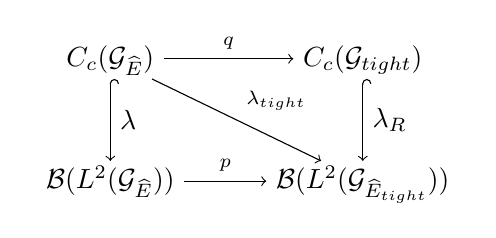
\begin{tikzpicture}
\matrix(m)[matrix of math nodes,row sep=3em, column sep=3em, text height=1.5ex, text depth = 0.25ex]
{C_{c}(\G_{\E})&C_{c}(\G_{tight})\\
\mathcal{B}(L^{2}(\G_{\E}))&\mathcal{B}(L^{2}(\G_{\E_{tight}}))\\};
\path[->,font=\scriptsize]
(m-1-1) edge node[auto] {$q$} (m-1-2)
(m-2-1) edge node[auto] {$p$} (m-2-2)
(m-1-1) edge node[auto] {$\lambda_{tight}$} (m-2-2);
\path[right hook->]
(m-1-1) edge node[auto] {$\lambda$} (m-2-1)
(m-1-2) edge node[auto] {$\lambda_{R}$} (m-2-2);

\end{tikzpicture}
\end{center}

where $\lambda_{R}$ is the left regular representation of $C_{c}(\G_{tight})$. It follows from the definition of $p$ that the bottom triangle commutes and the top triangle commutes as:
\begin{equation*}
\lambda_{x}(f) =\sum_{t \in \Max(S)} f_{t}(x)\lambda_{x}(1_{tt^{*}}\delta_{t}) = \lambda_{x}(qf)
\end{equation*}
For each $x \in \E_{tight}$. Hence:
\begin{equation*}
\Vert qf \Vert_{r} = \sup_{x \in \E_{tight}} \lbrace \Vert \lambda_{x}(qf) \Vert \rbrace = \sup_{x \in \E_{tight}} \lbrace \Vert \lambda_{x}(f) \Vert \rbrace \leq \Vert \lambda(f) \Vert = \Vert f \Vert_{r}
\end{equation*}
and so $q$ is contractive (and therefore continuous).
 
Now to consider (2). It is enough to compute the result of products of elements of the form $f_{s}\delta_{s}$ for some $s \in \Max(S)$. We then check the following two identities:


\begin{enumerate}[I]
\item $q(f_{s}\delta_{s} \ast f_{t}\delta_{t}) = q(f_{s}\delta_{s})\ast q(f_{t}\delta_{t})$
\item $(q(f_{s}\delta_{s}))^{*}=q((f_{s}\delta_{s})^{*})$
\end{enumerate}


To see (I) compute on a single element:
\begin{eqnarray*}
(f_{s}\delta_{s} \ast f_{t}\delta_{t})([st,\phi])=f_{s}(\theta_{t}(\phi))f_{t}(\phi)
\end{eqnarray*}
Apply $q$:
\begin{eqnarray*}
q(f_{s}\delta_{s} \ast f_{t}\delta_{t})([st,\phi])= (f_{s}\delta_{s} \ast f_{t}\delta_{t})|_{\E_{tight}}([st,\phi]) =f_{s}(\theta_{t}(\phi))f_{t}(\phi)
\end{eqnarray*}
For all $[st,\phi] \in \G_{\E_{tight}}$. Then compute the right hand side: 
\begin{eqnarray*}
(q(f_{s}\delta_{s}) \ast q(f_{t}\delta_{t}))([st,\phi])=f_{s}|_{\E_{tight}}(\theta_{t}(\phi))f_{t}|_{\E_{tight}}(\phi)
\end{eqnarray*}
Which matches for each $[st,\phi] \in \G_{\E_{tight}}$. 

To prove (II) we need to compute on a single element, where $(f_{s}\delta_{s})^{*}=\alpha_{s^{*}}(\overline{f_{s}})\delta_{s^{*}}$:

\begin{eqnarray*}
q((f_{s}\delta_{s})^{*})([s^{*},x])& = &\alpha_{s^{*}}(\overline{f_{s}})_{\E_{tight}}(x)\\
& = & \overline{f}(\theta_{s}(x)) \\ & = & \overline{f(\theta_{s}(x))} \\ & = & \overline{q(f)}(\theta_{s}(x)) \\ & = &  \alpha_{s^{*}}(\overline{q(f)})(x)
\end{eqnarray*}
Where the above holds for all $x \in \E_{tight}$ where the function $f_{s}$ is defined at $\theta_{s}(x)$ as required.

As $q$ is a continuous *-homomorphism, it extends to the completions.
\end{proof}

\subsection{Applying the machinery}
The following lemma is key in the proof of theorem \ref{thm:T1}.
\begin{lemma}\label{lem:L3}
Let $S$ be F-inverse and let $K \subset \Max(S)$ such that $K$ is finite and $T=\sum_{t \in K} a_{t}\lambda(1_{tt^{*}}\delta_{t})$ such that $a_{t}$ is the constant function that has value $a_{t}$ on $D_{tt^{*}}$. Then $\Vert T \Vert = \Vert qT \Vert$
\end{lemma}
\begin{proof}
It is immediate that $\Vert T \Vert \geq \Vert qT \Vert$ as $q$ is contractive. We arrive at the other inequality by applying Corollary (\ref{cor:C1}).
\begin{eqnarray*}
\Vert T \Vert_{L^{2}(\mathcal{G}_{x})} = \Vert \sum_{t \in K} a_{t}\lambda_{x}(1_{tt^{*}}\delta_{t}) \Vert = \Vert \sum_{t \in K} a_{t}Q_{x}\lambda_{\infty}(1_{tt^{*}}\delta_{t})Q_{x}^{*} \Vert \\
= \Vert Q_{x}(\sum_{t \in K} a_{t}\lambda_{\infty}(1_{tt^{*}}\delta_{t}))Q_{x}^{*} \Vert = \Vert Q_{x}(qT)Q_{x}^{*} \Vert \leq \Vert qT \Vert.
\end{eqnarray*}
This holds for every $x \in E$ and so by  $\Vert T \Vert = \Vert \lambda(T) \Vert = \sup \lbrace \Vert \lambda_{x}(T) \Vert : x \in E \rbrace \leq \Vert qT \Vert$. This gives the desired equality.  
\end{proof}

\begin{proof}

We know that we have a surjective *-homomorphism $q$ from $C^{*}_{r}(\G)$ to $C^{*}_{r}(G)$, we just need to see that the kernel of this map is $\overline{A}$. The set $\overline{A}$ is contained in the kernel as elements in $A$ are sums of functions with value at $1_{E}=\infty \in \widehat{E}$ of zero and projection onto this value (i.e applying q) will send the entire element to $0 \in C^{*}_{r}(G)$. So it is enough to show that $A$ is dense in the kernel.\\
\\
First consider finite sums. Let $f \in C_{c}(\mathcal{G})$. We need to show that if $qf=0$ then $ f \in A$.\\
\\
$f$ has the form:
\begin{equation*}
f=\sum_{s \in S} f_{s}\delta_{s} \mbox{ } f_{s}\in C(D_{ss^{*}})
\end{equation*}
With only finitely many non-zero terms. This can be viewed concretely on $L^{2}(\mathcal{G})$ using
\begin{equation*}
\lambda(f)=\sum_{s \in S} f_{s}\lambda(1_{ss^{*}}\delta_{s})
\end{equation*}
$S$ F-inverse allows us to reduce this sum using the following observation that for each $s \in S$ we can write the term $f_{s}\delta_{s}$ as $f_{s}\chi_{s}\delta_{t_{s}}$ where $t_{s}$ is the maximal element above $s$. So for each $t \in \Max(S)$ we can define $f^{'}_{t}=\sum_{s \leq t}f(s)\chi_{s}$ and then
\begin{equation}\label{Eq1}
\lambda(f)=\sum_{t \in \Max(S)} f^{'}_{t}\lambda(1_{tt^{*}}\delta_{t})
\end{equation}
(\ref{Eq1}) is in the kernel of $q$ if and only if each $f^{'}_{t}(\infty)=0$ for every $t \in \Max(S)$ that is if and only if $\lambda(f) \in A$.\\
\\
Now let $T$ be an element of $C^{*}_{r}(\G})$ such that $T$ is in the kernel of $q$ ($qT=0$). Then we need to show $T$ can be approximated by finite sums that lie in $A$. Let $T_{n}$ be finite sums in $C_{c}(\mathcal{G})$ with $T_{n} \rightarrow T$. Without loss of generality, these $T_{n}$ have the following form for some finite $K_{n} \subset \Max(S)$:
\begin{equation*}
T_{n}=\sum_{t \in K_{n}} f^{n}_{t}\lambda(1_{tt^{*}}\delta_{t})
\end{equation*}
then $qT_{n} = \sum_{t \in K_{n}} f^{n}_{t}(\infty)\lambda_{\infty}(1_{tt*}\delta_{t})$. Define a pullback of $qT_{n}$:
\begin{equation}
S_{n} = \sum_{t \in K_{n}} a^{n}_{t}\lambda(1_{tt*}\delta_{t}) \in C_{c}(\mathcal{G})
\end{equation}
Where $a^{n}_{t}$ is the constant function on $D_{tt^{*}}$ with value $f_{t}^{n}(\infty)$. It is clear that $qS_{n}=qT_{n}$ and using lemma \ref{lem:L3} we have that $\Vert S_{n} \Vert = \Vert qS_{n} \Vert = \Vert qT_{n} \Vert$ so $\Vert S_{n} \Vert \rightarrow 0$\\
\\
Let $U_{n}=(T_{n}-S_{n})$. Then $U_{n} \in A$ and $U_{n}=(T_{n}-S_{n}) \rightarrow (T-0)=T$, so T can be approximated by elements in $A$, hence $A$ is dense in $ker(q)$ and $\overline{A}=ker(q)$
\end{proof} 

\subsection{Translation algebras and a groupoid characterisation.}

Let $X$ be a uniformly discrete bounded geometry metric space.

\begin{definition}
The translation algebra associated with a partial translation structure $\mathcal{T}$ on $X$, denoted by $C^{*}\mathcal{T}$, is the completion as a *-subalgebra of $\mathcal{T}$ viewed as bounded operators on $\ell^{2}(X)$
\end{definition}

The aim of this section is to give a description of the partial translation algebra associated to a grouplike $\mathcal{T}$ with no zero divisors as the $C^{*}$-algebra of a groupoid, where the groupoid is related to the inverse monoid generated by the partial translations. We then recast a result of Brodzki, Niblo, Putwain and Wright \cite[Theorem 8.3]{Rosiesthesis} outlining a short exact sequence of $C^{*}$-algebras arising from such translation structures and compute some examples in certain cases.

The results in \cite[Theorem 1, Theorem 2]{MR2457037} allow us to draw the conclusion that the left regular representation of $S$ does not generate the correct covariant groupoid representation in general, however appears to match in the case of the Toeplitz algebra. This suggests that we are missing some information, but depending on the structure of the space this may not be necessary information. The information carried over from the partial translation structure that has not been used in this instance is the representation on $I(X)$, which determines a representation on $\ell^{2}(X)$ in the standard way. This representation will be the focus of this section. The following is \cite[Prop 10.6]{MR2419901}

\begin{proposition}\label{prop:P7} 
Let $\mu$ be a representation of $S$ on a Hilbert Space $H$. Then there exists a unique *-representation $\pi_{\mu}$ of $C_{0}(\E)$ on $H$ such that $\pi_{\mu}(1_{e})=\mu(e)$ for every $e \in E$ In addition $(\pi_{\mu} \times \mu)$ is a covariant representation for $\G_{\E}$. 
\end{proposition}
\begin{proof}
%Give a proof of this.
\end{proof}


The proof of the above result relies on the spectrum of the commutative $C^{*}$-subalgebra $A=C^{*}(E)$ of $C^{*}_{r}(S)$. We denote the spectrum by $\A$.

So given $X$ equipped with a grouplike partial translation structure with no zero divisors $\mathcal{T}$, we get an inverse monoid $S=\langle \mathcal{T} \rangle$ and a representation $\mu: S \hookrightarrow I_{b}(X)$ from Proposition \ref{prop:P6}. So applying Propsition \ref{prop:P7} we arrive at a representation $\pi_{\mu}$ of $C(\E)$ on $\ell^{2}(X)$. 

\begin{proposition}\label{prop:P9}
If $S$ is as above then the following hold for $\A$:
\begin{enumerate}
\item $\A \hookrightarrow \E$ is a topological embedding
\item $\beta X \twoheadrightarrow \A$ is a quotient map.
\end{itemize}
Moreover the topologies are all compatable with the topology endowed as the spectrum of $A=C^{*}(E)$.
\end{proposition}
\begin{proof}
First we show (1). From the proof of Proposition \ref{prop:P7} we see that we have a natural injective continuous map given by: 
\begin{equation*}
j: \psi \in \A \mapsto \phi = \psi \circ \sigma \in \E
\end{equation*}
$j(\A)$ is compact as j is continous and closed because $\E$ is Hausdorff.

For (2) we observe that the quotient map is given by the equivalence relation 
\begin{equation*}
\phi \sim \phi^{'} \leftrightarrow \phi \cap E(S) = \phi^{'} \cap E(S)
\end{equation*}
This map is surjective as given any $\psi \in \A$ we can view this as a filter on $X$ be considering the set:
\begin{equation*}
F_{\psi} = \lbrace e \in E(S) | \psi(\sigma(e))=1 \rbrace
\end{equation*}
We can complete this to an ultrafilter in $\beta X$ in many ways (Zorn's Lemma), however it is enough to show we can do it such that $F_{\psi ,UF}\cap E(S) = \psi$. So it is enough to pick subsets according to the following rules. Let $M,M^{c} \in \lbrace 0,1 \rbrace^{X}$ and
\begin{itemize}
\item If $M \in E(S)$ then add $M^{c}$ to $F_{\psi}$
\item If $M \not\in E(S)$ then add $M$ to $F_{\psi}$
\item If $M,M^{c} \not \in E(S)$ add either to $F_{\psi}$
\end{itemize}
With the case in which both $M$ and $M^{c}$ are contained in $E(S)$ is impossible as $E(S)$ has no zero element.

Now $F_{\psi}$ has the correct property and is an ultrafilter of $\beta X$ that maps onto $\psi$. Observe that the image of $\beta X$ is again compact, and thus closed, hence the map is a quotient.
\end{proof}

\begin{corollary}\label{cor:C3}
Let $\psi_{x} = \lbrace x \rbrace^{\uparrow} \cap E(S)$. Then the set $\lbrace \psi_{x} | x \in X \rbrace$ is dense in $\A$.
\end{corollary}

In the most general situation the subspace $X$ may be stabilized under the right or left action of the group; we denote the left stablizer $LStab_{G}(X)$ by $H$. 

\begin{proposition}\label{prop:P9a}
$x_{1}x_{2}^{-1} \in H \Leftrightarrow \forall t \in \mathcal{T} (x_{1} \in Dom(t) \Leftrightarrow x_{2} \in Dom(t))$
\end{proposition}
\begin{proof}
($\Rightarrow$) $x_{1}x_{2}^{-1} \in H$ is equivalent to $x_{1}, x_{2} \in Hx$ for some $x \in X$. This implies that $(x_{1} \in Dom(t) \Leftrightarrow x_{2} \in Dom(t))$ as the elements of $H$ are contranslations of $X$. 

In fact we can say that the elements of $H$ are precisely the cotranslations that are bijections of $X$. This is key in proving the converse:

($\Leftarrow$) Consider $h=x_{1}x_{2}^{-1}$. We want to see that for all $x \in X$ $hx \in X$. Observe that by the first property of translation structures there exists a unique translation $t$ such that $t(x_{2})=x$ Then $hx=ht(x_{2})=t(hx_{2})=t(x_{1}) \in X$ and this chain of equalities holds precisely when $(x_{1} \in Dom(t) \Leftrightarrow x_{2} \in Dom(t))$

\end{proof}

\begin{corollary}\label{cor:C5}
$B$ is in bijection with $H \backslash X$
\end{corollary}
\begin{proof}
The righthand side of Proposition \ref{prop:P9a} is equivalent to the condition that $\psi_{x_{1}}=\psi_{x_{2}} \in B$.
\end{proof}

It is immediate (using \cite[Prop 10.10]{MR2419901}) that the set $\A$ is invariant under the action of $S$. To compute the groupoid and groupoid $C^{*}$-algebras associated to $\A$ we would like to know a little more about the Hilbert spaces associated to the fibers and general connectness of the set $B:=\lbrace \psi_{x} | x \in X \rbrace$ (which using Corollary \ref{cor:C3} is dense in $\A$).

\begin{proposition}\label{prop:P10}
Let $t \in \mathcal{T}$. Then $\theta_{t}(\psi_{x})=\psi_{t(x)}$ for all $x \in Dom(t)$.
\end{proposition}
\begin{proof}
First some observations:
\begin{enumerate}
\item $\theta_{t}(\psi_{x})$ is defined as $\theta_{t}(\psi_{x}) \in D_{tt^{*}} \Leftrightarrow \psi_{x} \in D_{t^{*}t} \Leftrightarrow t^{*}t \in \psi_{x} \Leftrightarrow x \in t^{*}t = Dom(t)$.
\item $(\theta_{t}(\psi_{x}))(tet^{*})=\psi_{x}(t^{*}(tet^{*})t)=\psi_{x}(e)$. Hence $e \in \psi_{x} \Leftrightarrow tet^{*}  \in \theta_{t}(\psi_{x})$.
\item $\psi_{x}=\psi_{y} \Leftrightarrow \psi_{t(x)}=\psi_{t(y)}$, in fact more is true as: $\psi_{t(x)}=\psi_{t^{'}(y)} \Leftrightarrow Dom(t^{'})=Dom(t)$.
\end{enumerate}
We prove inclusions. First $\theta_{t}(\psi_{x}) \subset \psi_{t(x)}$. Without loss of generality, we can take $tet^{*}$ to be the general form of an element of $\theta_{t}(\psi_{x})$ and then: $tet^{*} \in \psi_{t(x)} \Leftrightarrow t(x) \in tet^{*} \Leftrightarrow tet^{*}(t(x))=t(x)$, which is the case if and only if $e \in \psi_{x}$.

To see the reverse inclusion let $f \in \psi_{t(x)}$. Then $f \in \theta_{t}(\psi_{x}) \Leftrightarrow t^{*}ft \in \psi_{x} \Leftrightarrow t(x) \in f \Leftrightarrow f \in \psi_{t(x)}$. 

To conclude; (3) controls the behavior of the action when the stabilizer is non-trivial, the first part shows the action behaves with respect to the quotient and the second part shows that given any pair $(x^{'},y^{'})\in X \times X$ such that $x^{'}\in Hx, y^{'}\in Ht(x)$ the unique translation $t_{x^{'}y^{'}} \in \mathcal{T}$ that sends $x^{'}$ to $y^{'}$ defines an arrow between $\psi_{x}$ and $\psi_{t(x)}$. 
\end{proof}

\begin{proposition}\label{cor:C4}
$B$ is invariant and $\G_{B}$ is connected. Moreover if $H$ is trivial, then $B$ is invariant and $\G_{B}$ is uniquely connected.
\end{proposition}
\begin{proof}
$B$ is invariant as a consequence of Proposition \ref{prop:P10}, and connected by the first property of grouplike partial translation structures - $\mathcal{T}$ partitions $X \times X$. This tells us that when we pass to the quotient $H \backslash X$ we get a collection of arrows between each pair of points that are indexed by $H$. 

In the situation that $H$ is trivial we get a unique arrow between any two points in $B$ and $B$ is in bijection with $X$, hence the groupoid $\G_{B}$ is precisely the pair groupoid $X \times X$, with the norm coming from the stalks, each of which have the form of $\ell^{2}(X)$ by the uniquely connected property of $B$.
\end{proof}

\begin{remark}
In the situation that $H$ is non-trivial, we have a unit space for $\G_{B}$ that is $B\times B$, with arrows between each pair indexed by $H$. The Hilbert space associated to each fibre $L^{2}(\G_{\A})|\psi_{x}$ is exactly the Hilbert space with basis indexed by the \textit{arrows} $[t_{h},\psi_{x}]$ - the set of arrows based at $\psi_{x}$ is in bijection with $X$, construct a map using the first property of translation structures.

For each point $hx \in Hx$ there exists a unique translation $t_{y,h}$ to each other point $y \in X$. We then define the map $[t_{y,h}, \psi_{x}] \mapsto t_{y,h}(hx)=y$.

This provides a unitary isomorphism between these spaces, denote this map at the level of Hilbert spaces by $U_{x}$ for each $x \in H \backslash X$.
\end{remark}

\begin{proposition}\label{prop:P11}
$\Vert \lambda(1_{tt^{*}}\delta_{t}) \Vert = \Vert \mu(t) \Vert_{\ell^{2}(X)}$ for all $t \in \mathcal{T}$. 
\end{propositon}
\begin{proof}
The proof of this fact follows from a computation on the basis of $\ell^{2}(X)$ using the unitary isomorphism $U_{x}$. We compute $U_{x}\lambda_{\psi_{x}}(1_{tt^{*}}\delta_{t})U_{x}^{-1}$ evaluated on a basis element $\delta_{y} \in \ell^{2}(X)$.
\begin{enumerate}
\item $U_{x}^{-1}(\delta_{y})=\delta_{[t_{y,h},\psi_{x}]}$
\item $\lambda_{\psi_{x}}(1_{tt^{*}}\delta_{t})(\delta_{[t_{y,h},\psi_{x}]})(\delta_{[s,\psi_{x}]})=\sum_{\substack{[n,\psi_{z}][u,\psi_{x}]\\=[s,\psi_{x}]}} 1_{tt^{*}}([n, \psi_{z}]\delta_{[t_{y,h},\psi_{x}]}([u,\psi_{x}])=\delta_{[t_{y,h},\psi_{x}]}$

Hence $\lambda_{\psi_{x}}(1_{tt^{*}}\delta_{t})$ moves the basis element $\delta_{[t_{y,h},\psi_{x}]}$ to the basis element $\delta_{[s,\psi_{x}]}$, where $s$ is the unique translation above $tt_{y,h}$ in $\mathcal{T}$. This is summarized in figure \ref{}.
\item $U_{x}(\delta_{[tt_{y,h},\psi_{x}]})=\delta_{t(t_{y,h}(hx))}=\delta_{t(y)}=\mu(t)(\delta_{y})$.
\end{enumerate}
This holds for all $y$ in the domain of $t$, as the multiplication in the groupoid is defined for only that situation.

As we have this equality for each $\psi_{x} \in B$; we get that $\Vert \lambda(1_{tt^{*}}\delta_{t}) \Vert_{r} = \sup \lbrace \Vert \lambda_{\psi_{x}}(1_{tt^{*}}\delta_{t}) \Vert : \psi_{x} \in B \rbrace = \Vert \mu(t) \Vert_{\ell^{2}(X)}$.
\end{proof}
\end{proposition}

This extends to finite sums:

\begin{lemma}\label{lem:L7}
Let $K \subset \A$ be a finite subset and let $a_{t}$ be the constant function valued $a_{t}$ on $D_{tt^{*}}$. Then \Vert \sum_{t \in K} a_{t}\delta_{t} \Vert_{r} = \Vert \sum_{t \in K} a_{t} \mu(t) \Vert_{\ell^{2}(X)}  
\end{lemma}
\begin{proof}

First we show that $\sum_{t \in K} a_{t}\delta_{t}$ represents as $\sum_{t \in K} a_{t} \mu(t)$ on the basis of $\ell^{2}(X)$. We proceed as in proposition \ref{prop:P10}. 

First compute $U_{x}^{-1}(\delta_{y})$:
\begin{equation*}
U_{x}^{-1}(\delta_{y})=\delta_{[t_{y,h},\psi_{x}]}
\end{equation*}
Then compute: 
\begin{eqnarray*}
(\sum_{t \in K}\lambda_{\psi_{x}}(a_{t}\delta_{t}))(\delta_{[t_{y,h},\psi_{x}]})& = &\sum_{\left\lbrace t\in K:\substack{[t,\psi_{y}][t_{y,h},\psi_{x}]\\=[tt_{y,h},\psi_{x}] }\right\rbrace} a_{t}([t, \psi_{y}])\delta_{[t_{y,h},\psi_{x}]}([t_{y,h},\psi_{x}])\\
& = &\sum_{\lbrace t \in K, y \in Dom(t)\rbrace }a_{t}([t,t_{y,h}(\psi_{x})])\delta_{[tt_{y,h}, \psi_{x}]}\\ & = &\sum_{t \in K,y \in Dom(t)}a_{t}\delta_{[tt_{y,h}, \psi_{x}]}
\end{eqnarray*}
Lastly move back to $\ell^{2}(X)$ via $U_{x}$:
\begin{eqnarray*}
U_{x}(\sum_{t \in K,y \in Dom(t)}a_{t}\delta_{[tt_{y,h}, \psi_{x}]}) & = &\sum_{t \in K, y \in Dom(t)}a_{t}\delta_{t(y)}\\ & = &(\sum_{t \in K}a_{t}\mu(t))(\delta_{y})
\end{eqnarray*}

\end{enumerate}

So both finite sums transform the basis in the same way. This equality holds for each $\psi_{x}$ in $B$, so we can conclude that $\Vert \sum_{t \in K} a_{t}\delta_{t} \Vert_{r} = \sup \lbrace \Vert \lambda_{\psi_{x}}(\sum_{t \in K} a_{t}\delta_{t} ) \Vert : \psi_{x} \in B \rbrace = \Vert \sum_{t \in K} a_{t} \mu(t) \Vert_{\ell^{2}(X)}$.
\end{proof}

This lets us define a map: 
\begin{equation*}
\mathcal{Q}: \lambda(1_{tt^{*}}\delta_{t}) \mapsto \mu(t)
\end{equation*}

Now we can state the main result of this section:
\begin{theorem}\label{thm:T5}
Let $X \subset G$, giving us a translation structure $\mathcal{T}_{G}|_{X}$ with no zero divisors and a representation $\mu: S = \langle \mathcal{T}_{G}|_{X} \rangle$. Then we have an isomorphism C^{*}_{r}(\G_{\A}) \cong C^{*}_{\mu}(S) = C^{*}\mathcal{T}. 
\end{theorem}

\begin{proof}
The map $\mathcal{Q}$ is surjective onto $\mathbb{C}S$ (mapping to the generators of $S$), so it remains to see that it passes to the completion and is injective. 
To show this, we appeal to Lemma \ref{lem:L7} to show that the norms match under the map $\mathcal{Q}$ up to finite sums - making the map on the incomplete algebras uniformly continous. Ideally, we would now complete - however we need to be careful as the incomplete *-algebra $M$ generated by finite sums of $1_{e}\delta_{t}$ may not be dense (and is the source of the map $\mathcal{Q}$).

To get over this obstruction we observe that by Stone-Weierstrass every element in $C(\A)$ can be approximated by elements of the form $1_{e}$, i.e for all $f_{t} \in C(\A)$:
\begin{equation*}
f_{t} = \lim_{n} (\sum_{e \in E} a^{n}_{e}1_{e})
\end{equation*}
So for a particular element  $f=\sum_{t \in K}f_{t}\delta_{t} \in C_{c}(\G_{\A})$ we can approximate each $f_{t}$ in turn by limits of $\sum_{e \in E} a_{e}1_{e}$ giving us an approximation by finite sums of elements in $M$. Hence $\overline{M} = C^{*}_{r}(\G_{\A})$, allowing $\mathcal{Q}$ to pass to completions (by uniform continuity).

After passing to the completion, the map is isometric; hence injective. This gives us the first isomorphism. To see the equality, observe that by definition the translation algebra is the algebra generated in $\mathcal{B}(\ell^{2}(X))$ by the set of operators $\lbrace \mu(t) | t \in \mathcal{T} \rbrace$. This is precisely $C^{*}_{\mu}(S)$.
\end{proof}

\subsection{A Short Exact Sequence of Translation Algebras}

In this situation we still have access to all the tools available in the general inverse monoid case, as well as all the geometric properties arising from the representation $\mu$.

\begin{theorem}\label{thm:T4}
Let $X \subset G$, $\mathcal{T}=\mathcal{T}_{G}|_{X}$ be a grouplike partial translation structure on $X$ with no zero divisors and $S=\langle \mathcal{T} \rangle \hookrightarrow_{\mu} I(X)$ be the associated F-inverse monoid. Then we have the following (intrinsic) short exact sequence of $C^{*}$-algebras:
\begin{equation}\label{eqn1}
0 \rightarrow C^{*}_{r}(\G_{U}|_{\A}) \rightarrow C^{*}_{r}(\G_{\A}) \rightarrow C^{*}_{r}(G) \rightarrow 0
\end{equation}
Where the middle term is the translation algebra associated to $X$ arising from $\mathcal{T}$
\end{theorem}
\begin{proof}
The proof follows the same lines as the proof of Theorem \ref{thm:T1}.
\begin{enumerate}
\item The map defined on finite sums still has the desired properties, i.e a finite sum is in the kernel if and only if all its components are 0.
\item We still have the same pullbacks of constant functions to the entire space; This enables the same construction of approximating elements; who each have the same norm control property provided by corollary \ref{cor:C1}.
\item We can then conclude that the kernel is the desired algebra (by density).
\end{enumerate}
\end{proof}

\subsection{Improving Theorem \ref{thm:T4}.}
In this section we outline a result of Milan and Steinberg \cite{} concerning decompositions of groupoid $C^{*}$-algebras using 

\begin{definition}
Let $G$ be a locally compact groupoid. Then we call a continuous homomorphism from $G$ to a locally compact group $\Gamma$ a group valued cocycle (or just cocycle).
\end{definition}

\begin{definition}
Let $\rho: G \rightarrow \Gamma$ be a cocycle. We say it is:
\begin{enumerate}
\item \textit{transverse} if the map $\Gamma \times G \rightarrow \Gamma \times X$, $(g, \gamma) \mapsto (g\rho(\gamma),s(\gamma))$ is open.
\item \textit{closed} if the map $\gamma \mapsto ((r(\gamma),\rho(\gamma),s(\gamma))$ is closed.
\item \textit{faithful} if the map $\gamma \mapsto ((r(\gamma),\rho(\gamma),s(\gamma))$ is injective.
\end{enumerate}
We call a cocycle $\rho$ with all these properties a \textit{(T,C,F)-cocycle}.
\end{definition}

From such a cocycle we can construct a locally compact Hausdorff $G$-space $Y$. The action is called the enveloping action of $\rho$ and is done as follows. Consider the space $\G^{(0)}\times \Gamma$, equipped with the product topology. Then define $\sim$ on $\G^{(0)}\times \Gamma$ by $(x,g)\sim (y,h)$ if there exists $\gamma \in \G$ with $s(\gamma)=x$, $r(\gamma)=y$ and $\rho(\gamma)=h^{-1}g$. We define $Y$ as the quotient of $\G^{(0)}\times \Gamma$ by $\sim$ with the quotient topology. The closed condition on the cocycle makes this space Hausdorff. We collect the main results of \cite{MR1900993}:

\begin{theorem}\label{Thm:1.8}
Let $\rho: \G \rightarrow \Gamma$ be a continuous, faithful, closed, transverse cocycle. Then the space $Y$ defined above is a locally compact Hausdorff space and there is a Morita equivalence of $\G$ with $Y\rtimes G$. Thus $C^{*}_{(r)}(\G)$ is strongly Morita equivalent to $C_{0}(Y)\rtimes_{(r)}\Gamma$. \qed
\end{theorem}

What follows from here can be found as a corollary to \cite[Theorem 6.14]{Milan-Steinberg}. We provide a direct proof of a special case using the original methods of \cite{MR1900993}. This is possible by considering the construction of the groupoid $G(S)$ for a strongly 0-E-unitary inverse monoid $S$. It is clear that the only danger is mapping elements to $0$ in $\Gamma^{0}$; this is overcome by the observation that the element $[0,f]$ would be defined if and only if $f \in D_{0}$. However, $f \in D_{0}$ implies that $f(0)=1$ and hence $f \not\in \E$, so the $0$ element of $S$ contributes nothing to the groupoid $G(S)$, either in objects or arrows.

\begin{theorem}
Let $S$ be an inverse monoid. If $S$ is strongly 0-E-unitary with universal group $U(S)=\Gamma$ such that the prehomomorphism has the finite cover property. Then the groupoid $G(S)$ admits a transverse and faithful cocycle to a group.
\end{theorem}
\begin{proof}
Let $\Phi$ be the 0-restricted, idempotent pure prehomomorphism onto $\Gamma^{0}$. We build an induced map on the groupoid $G(S)$ by considering a new map $\Psi:$
\begin{equation*}
\Psi([s,x])=\Phi(s)
\end{equation*}
This map is well-defined as any non-zero idempotent in $S$ is mapped to the identity in $\Gamma$, and so for any pair $(s,f) \sim (t,f)$ there is an $e \in E \cap D_{f}$, in particular not $0$, such that $es=et$ and hence $\Phi(s)=\Phi(es)=\Phi(et)=\Phi(t)$. This is clearly a groupoid homomorphism to $\Gamma$. To check it is continuous observe that as $\Gamma$ is a discrete group so all subsets are open. The preimage of a singleton is given by the union:
\begin{equation*}
\Psi^{-1}(\lbrace g \rbrace)=\bigcup_{\Phi(u)=g}[u,D_{u^{*}u}] 
\end{equation*}
which is certainly open in $G(S)$. The map is proper, because the preimage of any finite set in $\Gamma$ is given by a finite union of $[u,D_{u^{*}u}]$ that are compact by construction.

It remains to check it is a (T,C,F)-cocycle, and from the remarks prior to the Theorem the proof of this follows exactly from the proof \cite[Proposition 3.6]{MR1900993} modified suitably. We provide this proof below:

To prove this is transverse, it is enough to prove that $\lbrace (\Psi(\gamma),s(\gamma)):\gamma \in G(S)\rbrace$ is open in $\Gamma \times G(S)^{(0)}$, and this in turn reduces to studying this problem for all $g \in G$, that is if $\lbrace s(\gamma) :\Psi(\gamma)=g \rbrace$. is open in $G(S)^{(0)}$. This set is equal to $\bigcup_{\Psi(\gamma)=g}D_{s(\gamma)}$, which is certainly open in $G(S)^{(0)}$ as each piece is.

To see that this is faithful, let $[u,f], [v,f^{'}] \in G(S)$ such that $(f,\Phi(u),\theta_{u}(f))=(f^{'},\Phi(v),\theta_{v}(f^{'}))$. Then it is clear that $f=s([u,f])=s([v,f^{'}])=f^{'}$, so it is enough to prove now that $\Phi(v)=\Phi(u)$ implies $[u,f]=[v,f]$. Observe that $\Phi(u)\Phi(v)^{-1}=1$ in $\Gamma$ and $\Phi(v)^{-1}=\Phi(v^{*})$, so $\Phi(uv^{*})=1$. This map is idempotent pure, so $uv^{*} \in E(S)$. So $[u,f][v,f]^{-1}=[uv^{*},\theta_{v}(f)]$ is a unit in $G(S)$. From here it is clear that $[u,f]$ is an inverse to $[v^{*},\theta_{v}(f)]$ and so $[u,f]=[v,f]$.\end{proof}

This gets us a little closer to applying Theorem \ref{thm:1.8}. We still need to check the fact that the cocycles are closed. We proceed as in \cite{MR1900993}.

\begin{definition}
We say that S satisfies the finite cover property with respect to $\phi$,, if for every $p,q \in S$, $p,q\not = 0$ there exists a finite set $U \subset S_{g}$ such that:
\begin{equation*}
pS_{g}q=\lbrace s \in S | \exists u \in U | s \leq u \rbrace.
\end{equation*}
Where $S_{g}$ is the preimage $\phi^{-1}(g)$.
\end{definition}

Again, this follows from the work of \cite{Milan-Steinberg} or \cite{MR1900993}, but we give the proof in this setting:

\begin{lemma}
If $S$ is an inverse monoid and has the finite cover property with respect to $\phi$, then the induced cocycle $\rho$ is closed.
\end{lemma}
\begin{proof}
As $\Gamma$ is discrete, it is enough to prove that the graph $Gr(g)$ over $g$ in $G(S)^{(0)}\times G(S)^{(0)}$ is closed. We remark also that this product space is covered by the set of $D_{e} \times D_{f}$, where $e,f$ run though the idempotents $E(S)$, and is compact; thus only finitely many pairs $D_{e}\times D_{f}$ are necessary. The intersection $Gr(g) \cap D_{e}\times D_{f}$ is covered by $\bigcup_{u \in eS_{g}f} [u,D_{u^{*}u}]$ and so are compact if and only if:
\begin{equation*}
Gr(g) \cap D_{e}\times D_{f} = \bigcup_{u \in U}[u,D_{u^{*}u}]
\end{equation*}
for some finite $U \subset S_{g}$. However, this is precisely implied by the finite cover property.
\end{proof}

\begin{corollary}\label{Thm:Trick}
If $S$ is a 0-E-unitary monoid with the finite cover property then the groupoid $G(S)$ is Morita equivalent a transformation groupoid $Y \rtimes G$.\qed
\end{corollary}

\begin{remark}
If, in addition the inverse monoid $S$ is 0-F-inverse, then it satisfies the finite cover property with $\vert U \vert=1$, as each $S_{g}$ will contain a unique maximal element, and hence so will any truncation.
\end{remark}

Say something smart here...

\begin{theorem}
Let $S$ be a strongly $0$-F-inverse monoid with universal group $U(S)$. If $U(S)$ is $K$-exact then the short exact sequence:
\begin{equation*}

\end{equation*}
is exact at the level of K-theory.  
\end{theorem}

\section{Applications.}

\subsection{Pimsner-Voiculescu and K-theory.}

\subsection{Semigroup $C^{*}$-algebras and the Baum-Connes conjecture for subsemigroups of groups.}

\bibliography{ref.bib}

\end{document}